\subsection{Additional Results}
\label{app:additional-results}

\subsubsection{Adapter ablation}
\label{app:adapter}

Table~\ref{tab:adapter-ablation} gives the full Gate 4a comparison. Figure~\ref{fig:adapter-ablation} visualizes the same test MSE values. The missingness-aware FiLM branch is active, but it does not outperform the static adapter.

\begin{table}[ht]
    \centering
    \caption{Gate 4a adapter comparison on ETTh1 random-0.3.}
    \label{tab:adapter-ablation}
    \scriptsize
    \begin{tabular}{@{}lrrrrrr@{}}
\toprule
Variant & Trainable & Overhead & Best epoch & Val. MSE & Test MSE & Test MAE \\
\midrule
Official & 0 & 0.00\% & NA & NA & 0.425394 & 0.450336 \\
Static adapter & 33,600 & 2.96\% & 1 & 0.678666 & 0.361377 & 0.390458 \\
Missingness-aware FiLM adapter & 39,136 & 3.44\% & 5 & 0.679754 & 0.363156 & 0.391077 \\
\bottomrule
\end{tabular}

\end{table}

\begin{figure}[ht]
    \centering
    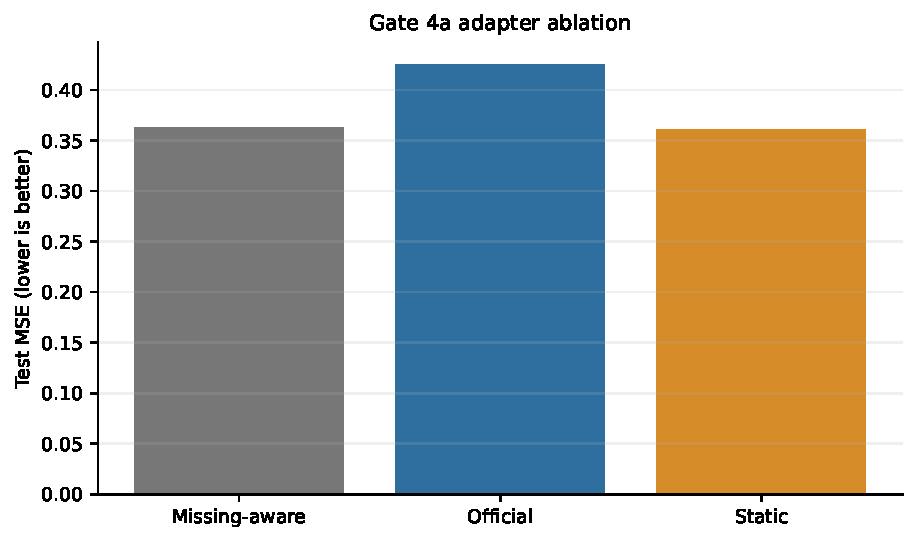
\includegraphics[width=0.78\linewidth]{figures/figA1_gate4a_adapter.pdf}
    \caption{Static and missingness-aware adapter results relative to the official reference.}
    \label{fig:adapter-ablation}
\end{figure}

\subsubsection{Cross-condition TimePerceiver evidence}

Table~\ref{tab:etth1-cross-condition} reports the ETTh1 condition matrix. It uses the same fixed evaluation assets for Gaussian and Student-$t$ heads within each condition.

\begin{table}[ht]
    \centering
    \caption{ETTh1 cross-condition paired comparison.}
    \label{tab:etth1-cross-condition}
    \scriptsize
    \resizebox{\linewidth}{!}{\begin{tabular}{@{}lrrrrrr@{}}
\toprule
Condition & $\Delta$NLL & $\Delta$CRPS & $\Delta$MSE & NLL win & CRPS NI & Point NI \\
\midrule
Random 0.1 & -0.078025 & -0.006113 & -0.002231 & Yes & Yes & Yes \\
Random 0.3 & -0.041381 & -0.003864 & -0.001155 & Yes & Yes & Yes \\
Random 0.5 & -0.013720 & 0.000656 & 0.007100 & Yes & No & No \\
Block 0.3 & -0.061086 & -0.007738 & -0.004834 & Yes & Yes & Yes \\
Channel 0.3 & -0.071504 & -0.004849 & 0.001022 & Yes & Yes & Yes \\
Mixed 0.3 & -0.070665 & -0.003286 & 0.001169 & Yes & Yes & Yes \\
\bottomrule
\end{tabular}
}
\end{table}

\subsubsection{Conformal details}

Tables~\ref{tab:conformal-main} and~\ref{tab:conformal-mechanism} retain the formal conformal results and mechanism audit. Figure~\ref{fig:calibration-shift} compares calibration and test coverage. Figures~\ref{fig:channel-coverage} and~\ref{fig:horizon-coverage} show channel- and horizon-level diagnostics.

\begin{table}[ht]
    \centering
    \caption{Formal additive conformal results.}
    \label{tab:conformal-main}
    \scriptsize
    \begin{tabular}{@{}lrrrrr@{}}
\toprule
Method & Nominal & PICP & MPIW & Coverage error & Interval score \\
\midrule
Mask-severity-conditioned conformal & 0.90 & 0.927136 & 2.262613 & 0.027136 & 2.989775 \\
Marginal conformal & 0.90 & 0.927636 & 2.267989 & 0.027636 & 2.990528 \\
Native & 0.90 & 0.897581 & 1.953189 & 0.002419 & 2.946898 \\
Mask-severity-conditioned conformal & 0.95 & 0.964262 & 2.993500 & 0.014262 & 3.625242 \\
Marginal conformal & 0.95 & 0.964505 & 2.998730 & 0.014505 & 3.625259 \\
Native & 0.95 & 0.937700 & 2.424187 & 0.012300 & 3.596873 \\
\bottomrule
\end{tabular}

\end{table}

\begin{table}[ht]
    \centering
    \caption{Conformal mechanism audit. Counterfactual values are diagnostic and not formal calibration.}
    \label{tab:conformal-mechanism}
    \scriptsize
    \resizebox{\linewidth}{!}{\begin{tabular}{@{}lrrrrrr@{}}
\toprule
Head & Nominal & Cal. PICP & Test PICP & Shift & $\hat q$ & $\Delta$ coverage error \\
\midrule
Gaussian & 0.90 & 0.869114 & 0.904533 & 0.035418 & 0.126842 & 0.023728 \\
Gaussian & 0.95 & 0.912017 & 0.937263 & 0.025246 & 0.279881 & 0.001974 \\
Student-t & 0.90 & 0.861667 & 0.897581 & 0.035913 & 0.157400 & 0.025216 \\
Student-t & 0.95 & 0.913178 & 0.937700 & 0.024522 & 0.287271 & 0.002205 \\
\bottomrule
\end{tabular}
}
\end{table}

\begin{figure}[ht]
    \centering
    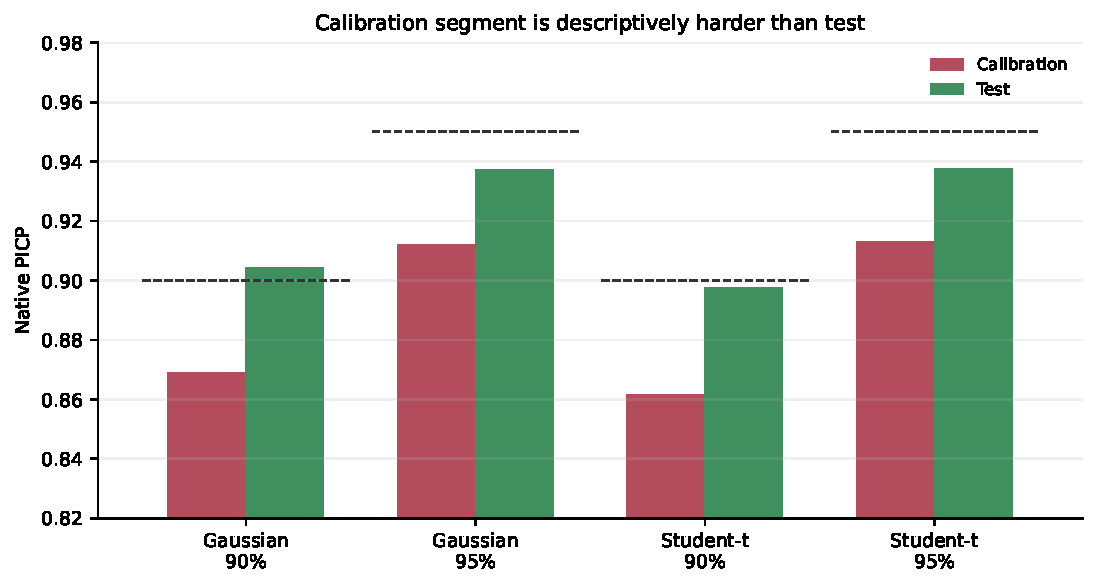
\includegraphics[width=0.78\linewidth]{figures/fig6_calibration_test_shift.pdf}
    \caption{Descriptive calibration-to-test coverage shift under the strict temporal split.}
    \label{fig:calibration-shift}
\end{figure}

\begin{figure}[ht]
    \centering
    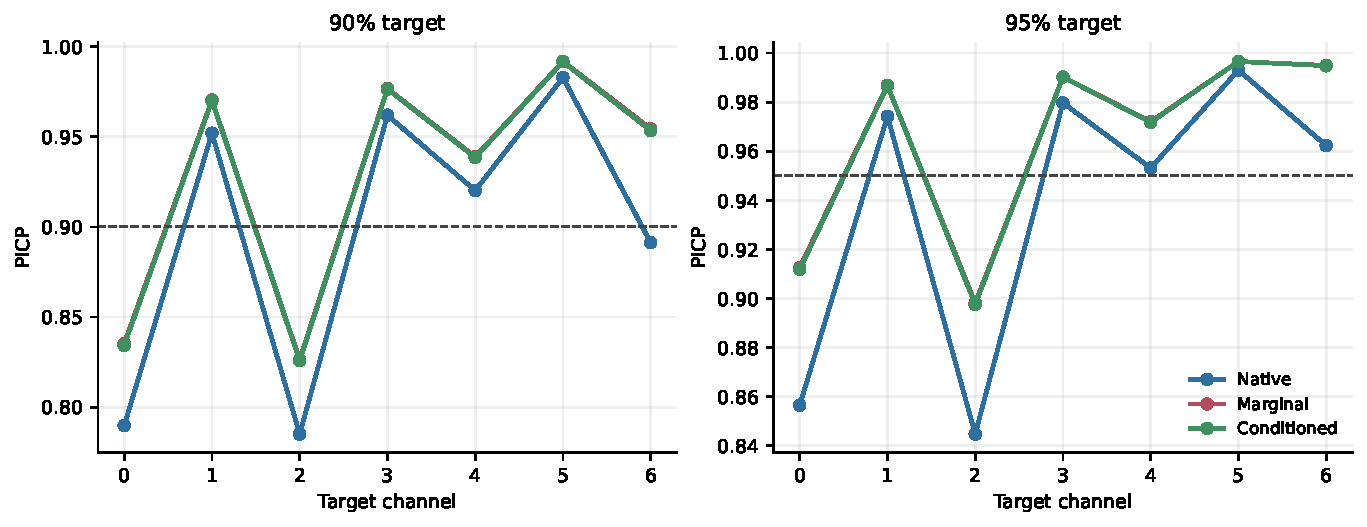
\includegraphics[width=0.48\linewidth]{figures/figA2_gate4c_channel_coverage.pdf}
    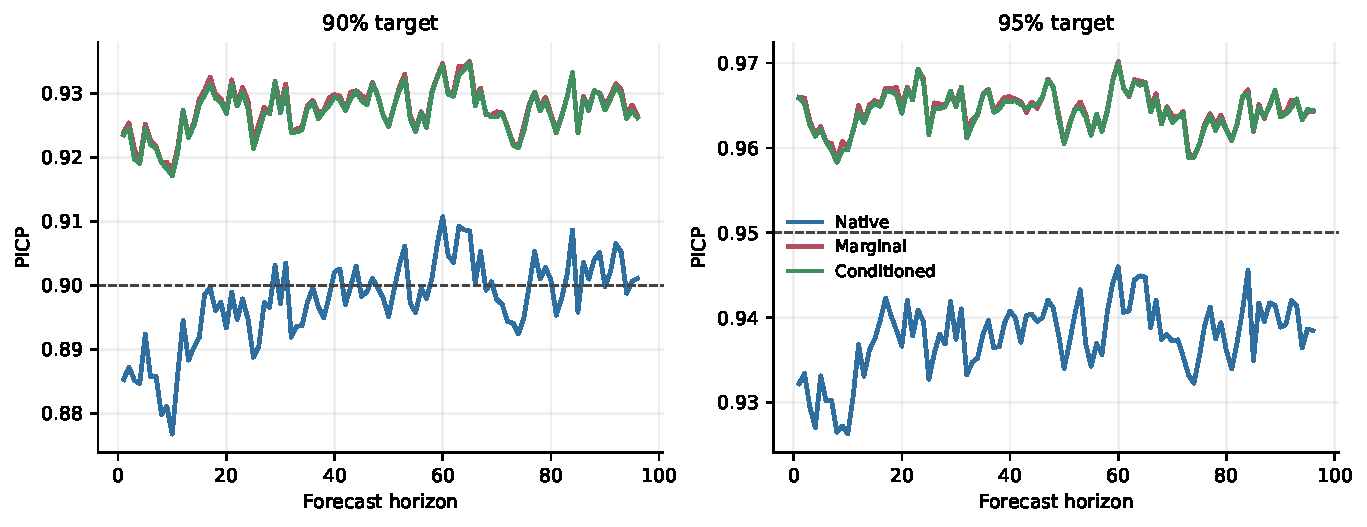
\includegraphics[width=0.48\linewidth]{figures/figA3_gate4c_horizon_coverage.pdf}
    \caption{Channel-level and horizon-level coverage diagnostics for the Gate 4c experiment.}
    \label{fig:channel-coverage}
    \label{fig:horizon-coverage}
\end{figure}

\subsubsection{Complete fixed-mask degradation matrix}

Tables~\ref{tab:full-mask-etth1}--\ref{tab:full-mask-electricity} retain every Gate 3b cell while splitting the matrix by dataset for readability.

\begin{table}[ht]
    \centering
    \caption{Full ETTh1 fixed-mask degradation matrix.}
    \label{tab:full-mask-etth1}
    \scriptsize
    \begin{tabular}{@{}lrrrr@{}}
\toprule
Mask & Rate & MSE & MAE & RMSE \\
\midrule
Block & 0.10 & 0.388818 & 0.416915 & 0.623552 \\
Block & 0.30 & 0.423837 & 0.451188 & 0.651027 \\
Block & 0.50 & 0.486504 & 0.501242 & 0.697498 \\
Block & 0.70 & 0.591697 & 0.571655 & 0.769219 \\
Channel & 0.10 & 0.479410 & 0.455063 & 0.692394 \\
Channel & 0.30 & 0.583704 & 0.511084 & 0.764006 \\
Channel & 0.50 & 0.798862 & 0.627325 & 0.893791 \\
Channel & 0.70 & 0.900947 & 0.683061 & 0.949182 \\
Mixed & 0.10 & 0.486209 & 0.464128 & 0.697287 \\
Mixed & 0.30 & 0.495055 & 0.473908 & 0.703601 \\
Mixed & 0.50 & 0.553485 & 0.525226 & 0.743966 \\
Mixed & 0.70 & 0.715806 & 0.617339 & 0.846053 \\
Random & 0.10 & 0.378811 & 0.408069 & 0.615476 \\
Random & 0.30 & 0.425394 & 0.450336 & 0.652223 \\
Random & 0.50 & 0.525856 & 0.523115 & 0.725160 \\
Random & 0.70 & 0.688520 & 0.617690 & 0.829771 \\
\bottomrule
\end{tabular}

\end{table}

\begin{table}[ht]
    \centering
    \caption{Full Weather fixed-mask degradation matrix.}
    \label{tab:full-mask-weather}
    \scriptsize
    \begin{tabular}{@{}lrrrr@{}}
\toprule
Mask & Rate & MSE & MAE & RMSE \\
\midrule
Block & 0.10 & 0.158302 & 0.218956 & 0.397872 \\
Block & 0.30 & 0.180420 & 0.245178 & 0.424759 \\
Block & 0.50 & 0.210474 & 0.277453 & 0.458774 \\
Block & 0.70 & 0.254572 & 0.322297 & 0.504551 \\
Channel & 0.10 & 0.191289 & 0.238851 & 0.437366 \\
Channel & 0.30 & 0.284471 & 0.316355 & 0.533358 \\
Channel & 0.50 & 0.377902 & 0.393866 & 0.614738 \\
Channel & 0.70 & 0.495709 & 0.490618 & 0.704066 \\
Mixed & 0.10 & 0.175815 & 0.230739 & 0.419303 \\
Mixed & 0.30 & 0.224939 & 0.281431 & 0.474278 \\
Mixed & 0.50 & 0.306930 & 0.357264 & 0.554012 \\
Mixed & 0.70 & 0.400193 & 0.440502 & 0.632608 \\
Random & 0.10 & 0.169631 & 0.232543 & 0.411863 \\
Random & 0.30 & 0.240810 & 0.309629 & 0.490724 \\
Random & 0.50 & 0.331313 & 0.391138 & 0.575598 \\
Random & 0.70 & 0.434543 & 0.474367 & 0.659199 \\
\bottomrule
\end{tabular}

\end{table}

\begin{table}[ht]
    \centering
    \caption{Full Electricity fixed-mask degradation matrix.}
    \label{tab:full-mask-electricity}
    \scriptsize
    \begin{tabular}{@{}lrrrr@{}}
\toprule
Mask & Rate & MSE & MAE & RMSE \\
\midrule
Block & 0.10 & 0.143247 & 0.243795 & 0.378480 \\
Block & 0.30 & 0.184630 & 0.289155 & 0.429686 \\
Block & 0.50 & 0.270835 & 0.369677 & 0.520418 \\
Block & 0.70 & 0.464169 & 0.520260 & 0.681300 \\
Channel & 0.10 & 0.213972 & 0.281108 & 0.462571 \\
Channel & 0.30 & 0.391038 & 0.403166 & 0.625331 \\
Channel & 0.50 & 0.569116 & 0.525639 & 0.754398 \\
Channel & 0.70 & 0.748916 & 0.649662 & 0.865399 \\
Mixed & 0.10 & 0.165759 & 0.254616 & 0.407135 \\
Mixed & 0.30 & 0.246785 & 0.325159 & 0.496775 \\
Mixed & 0.50 & 0.375182 & 0.437690 & 0.612521 \\
Mixed & 0.70 & 0.588662 & 0.596810 & 0.767243 \\
Random & 0.10 & 0.138429 & 0.242728 & 0.372060 \\
Random & 0.30 & 0.200572 & 0.318891 & 0.447853 \\
Random & 0.50 & 0.325732 & 0.432183 & 0.570729 \\
Random & 0.70 & 0.546080 & 0.584678 & 0.738972 \\
\bottomrule
\end{tabular}

\end{table}

\subsubsection{All conformal heads}

Table~\ref{tab:all-conformal-heads} reports every retained head and interval method. Extra probability diagnostics are shown in Figures~\ref{fig:pit-diagnostic}--\ref{fig:patchtst-tail}.

\begin{table}[ht]
    \centering
    \caption{All Gate 4c head and interval-method combinations.}
    \label{tab:all-conformal-heads}
    \scriptsize
    \resizebox{\linewidth}{!}{\begin{tabular}{@{}lrrrrrr@{}}
\toprule
Head & Method & Nominal & PICP & MPIW & Coverage error & Interval score \\
\midrule
Gaussian & Mask-severity-conditioned conformal & 0.90 & 0.927797 & 2.289391 & 0.027797 & 2.979145 \\
Gaussian & Marginal conformal & 0.90 & 0.928261 & 2.294196 & 0.028261 & 2.979930 \\
Gaussian & Native & 0.90 & 0.904533 & 2.040512 & 0.004533 & 2.936425 \\
Gaussian & Mask-severity-conditioned conformal & 0.95 & 0.964530 & 2.986506 & 0.014530 & 3.598434 \\
Gaussian & Marginal conformal & 0.95 & 0.964711 & 2.991181 & 0.014711 & 3.598406 \\
Gaussian & Native & 0.95 & 0.937263 & 2.431420 & 0.012737 & 3.571486 \\
Student-t & Mask-severity-conditioned conformal & 0.90 & 0.927136 & 2.262613 & 0.027136 & 2.989775 \\
Student-t & Marginal conformal & 0.90 & 0.927636 & 2.267989 & 0.027636 & 2.990528 \\
Student-t & Native & 0.90 & 0.897581 & 1.953189 & 0.002419 & 2.946898 \\
Student-t & Mask-severity-conditioned conformal & 0.95 & 0.964262 & 2.993500 & 0.014262 & 3.625242 \\
Student-t & Marginal conformal & 0.95 & 0.964505 & 2.998730 & 0.014505 & 3.625259 \\
Student-t & Native & 0.95 & 0.937700 & 2.424187 & 0.012300 & 3.596873 \\
\bottomrule
\end{tabular}
}
\end{table}

\begin{figure}[ht]
    \centering
    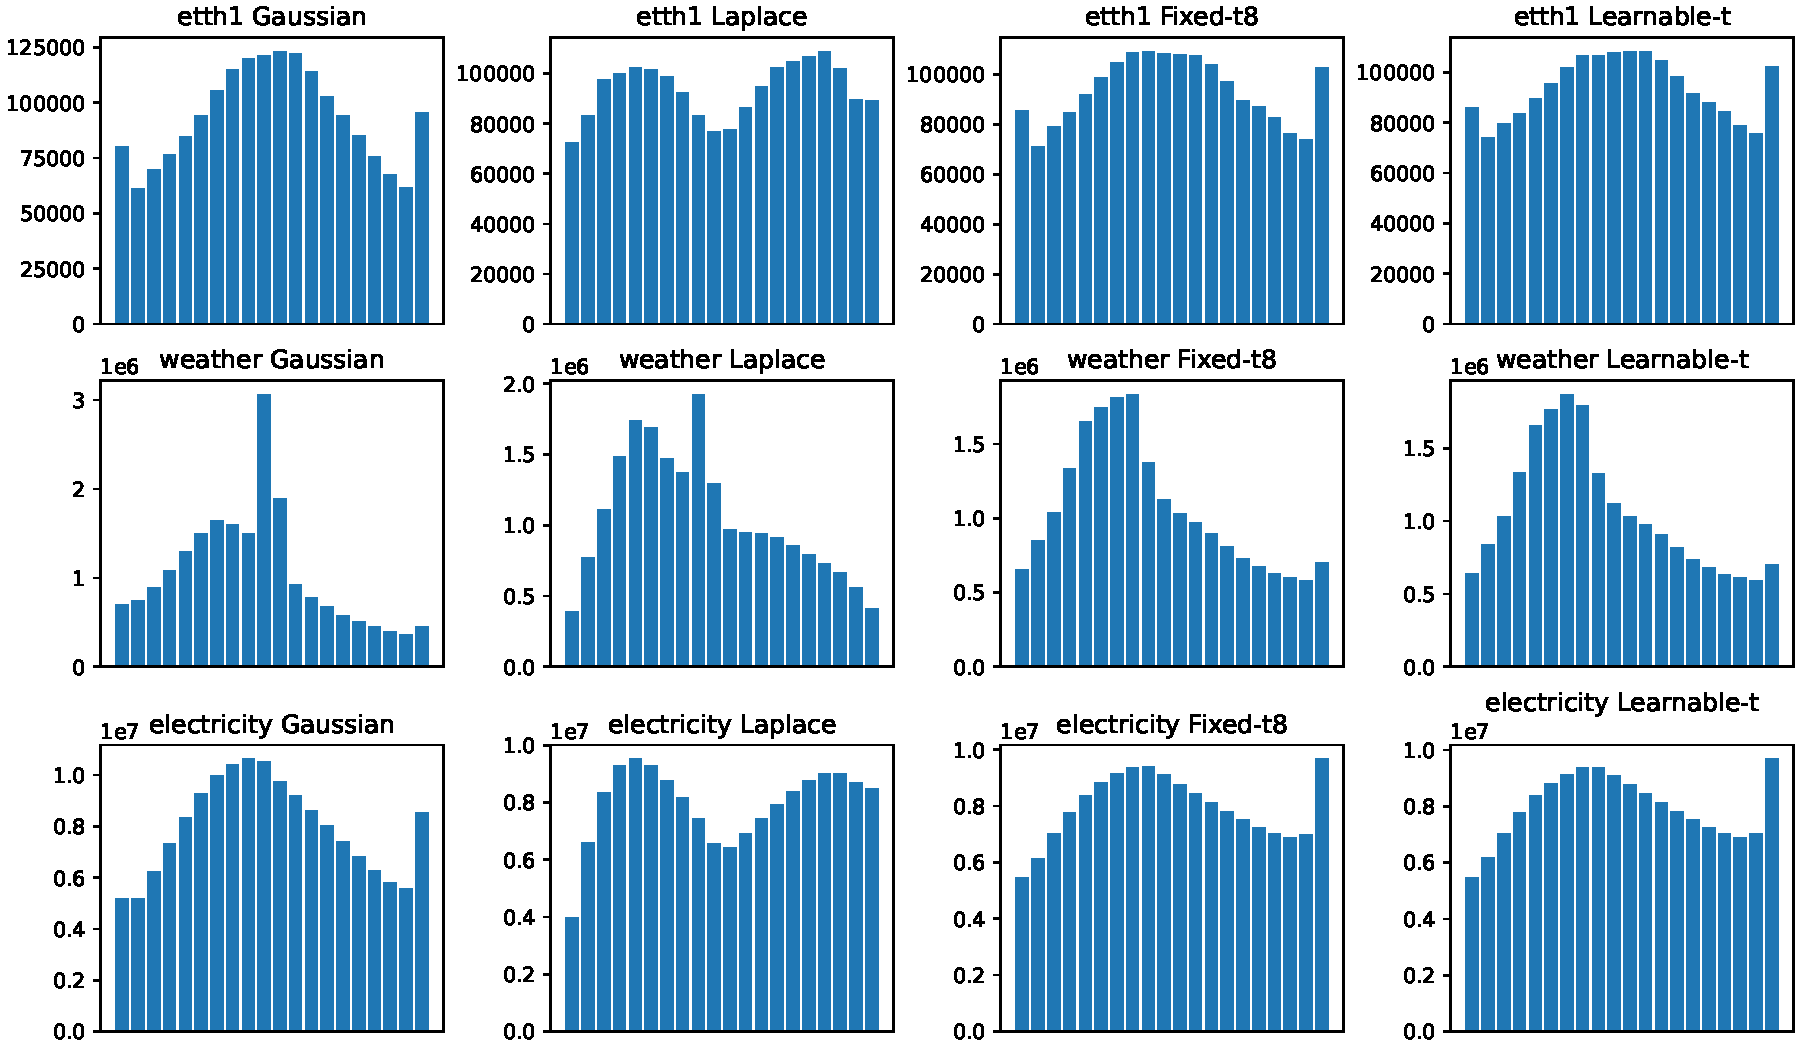
\includegraphics[width=0.48\linewidth]{figures/fig_gate5a_pit_histograms.pdf}
    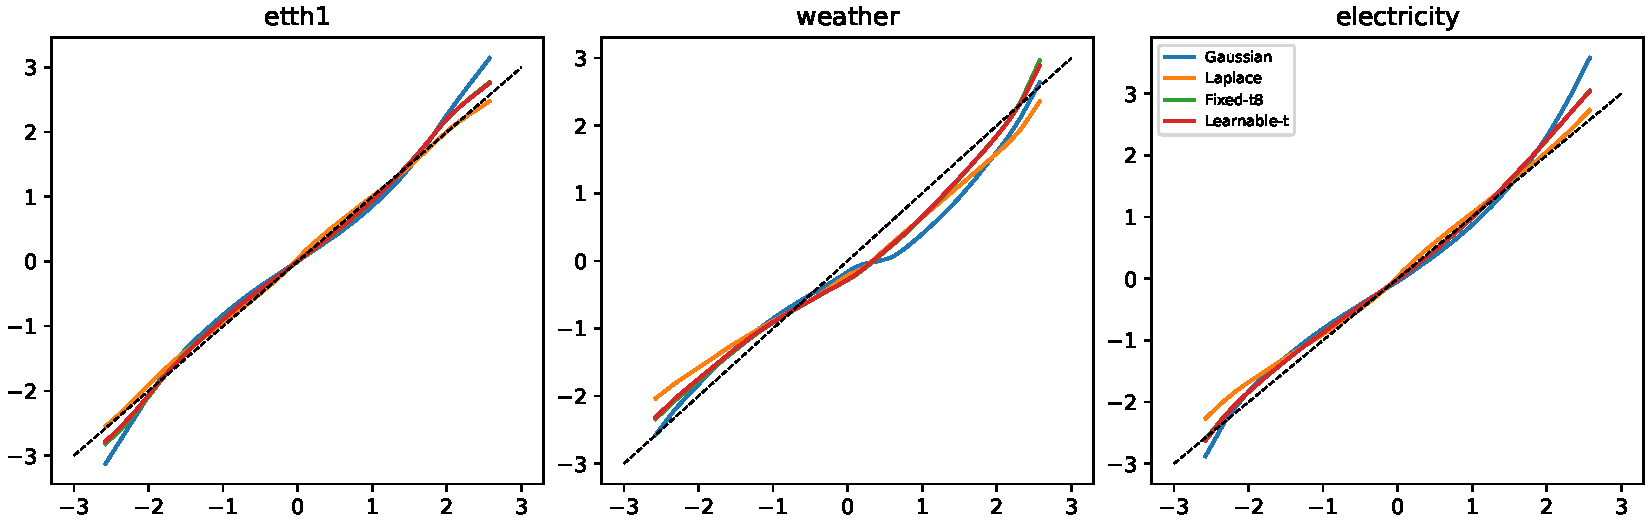
\includegraphics[width=0.48\linewidth]{figures/fig_gate5a_qq.pdf}
    \caption{Descriptive probability integral transform and quantile diagnostics.}
    \label{fig:pit-diagnostic}
\end{figure}

\begin{figure}[ht]
    \centering
    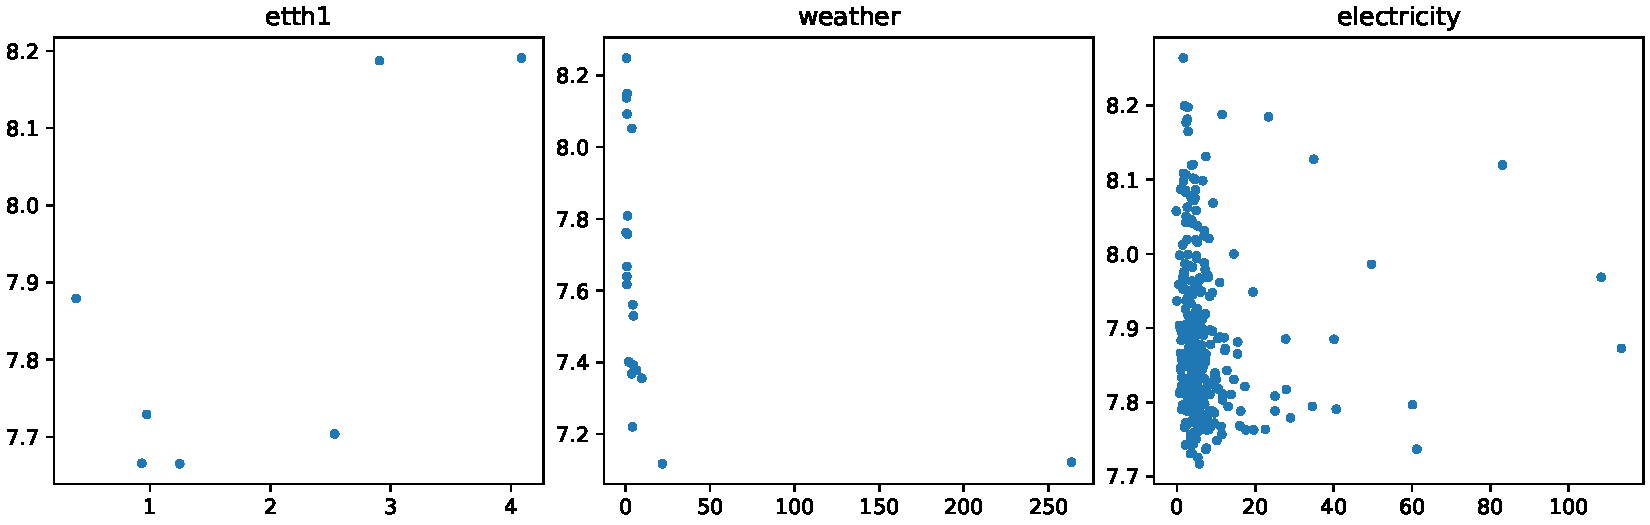
\includegraphics[width=0.48\linewidth]{figures/fig_gate5a_kurtosis_df.pdf}
    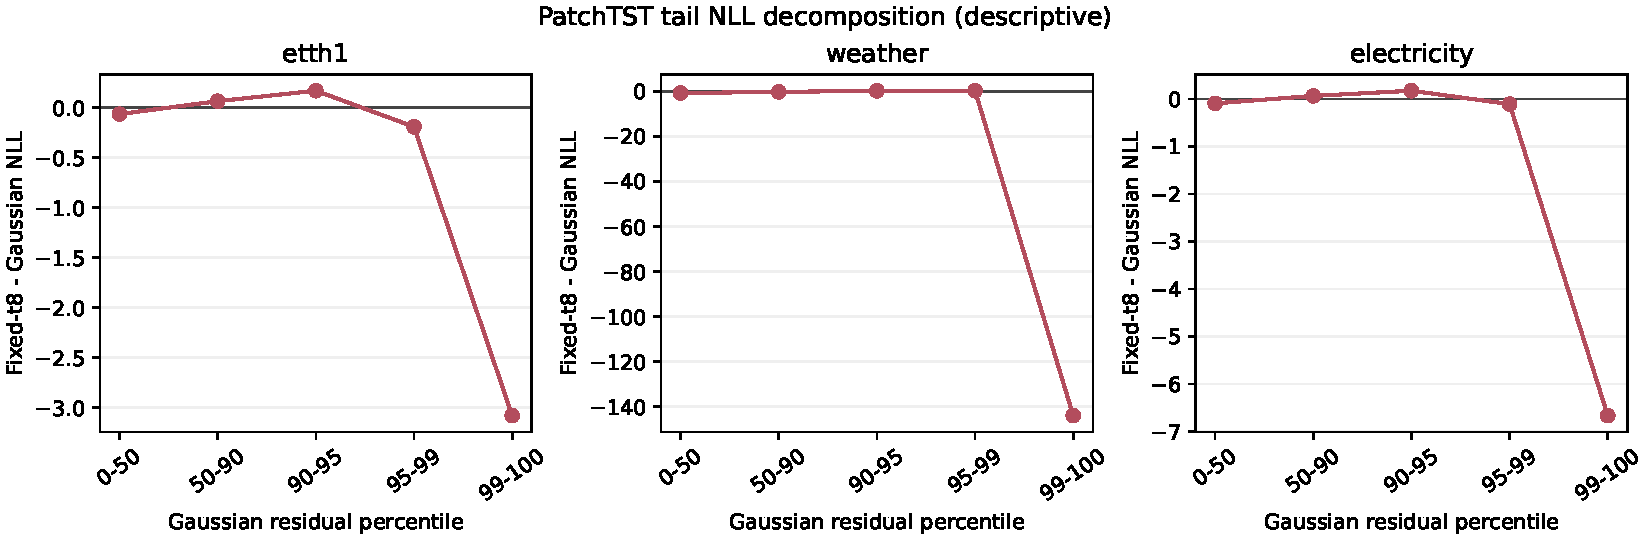
\includegraphics[width=0.48\linewidth]{figures/fig_gate5b_patchtst_tail_nll_gain.pdf}
    \caption{Channel-tail diagnostics and the descriptive PatchTST residual-percentile NLL decomposition.}
    \label{fig:patchtst-tail}
\end{figure}
